% Bản tiếng Việt đầy đủ để phản biện; giữ cùng claim, bảng, hình và tài liệu tham khảo với bản Anh.
\documentclass[conference]{IEEEtran}
\IEEEoverridecommandlockouts
\usepackage{fontspec}
\setmainfont{Times New Roman}
\setsansfont{Arial}
\setmonofont{DejaVu Sans Mono}
\usepackage{graphicx}
\graphicspath{{figures/}}
\usepackage{amsmath,amssymb}
\usepackage{booktabs}
\usepackage{array}
\usepackage{url}
\usepackage{balance}
\usepackage{microtype}
\linespread{0.97}

\title{AEB Radar-Only, Camera-Gated và Emergency-Fallback: Đánh đổi theo tình huống và mức độ nghiêm trọng của lỗi trong CARLA}

\author{
\IEEEauthorblockN{Mai Việt Hoàng và Phạm Đức An}
\IEEEauthorblockA{\textit{Đại học Bách khoa Hà Nội}\\
Hà Nội, Việt Nam\\hoangmai04222@gmail.com}
}

\begin{document}
\maketitle

\begin{abstract}
Camera permission gate có thể chặn phanh nhầm do radar nhưng đồng thời phủ quyết
vật cản nằm ngoài không gian nhãn của detector. Bài báo so sánh radar-only, hard
camera gate và camera gate có radar emergency fallback trong pipeline phanh khẩn
cấp tự động (AEB) sensor-to-brake trên CARLA 0.9.11. Khác với phân tích theo số
lượt chạy, đơn vị chính là named condition: 105 điều kiện core và frozen adverse
hold-out 14 điều kiện; mỗi điều kiện lặp năm lần chỉ để kiểm tra consistency.
Trên core, radar-only, hard gate và fallback lần lượt đạt precision/recall theo
điều kiện là 0,913/0,988, 1,000/0,965 và 1,000/0,988; fallback PASS 101/105 điều
kiện. Kết quả này không khái quát thành dominance. Hard gate PASS 11/14 điều
kiện hold-out so với 7/14 của fallback vì bốn điều kiện synthetic ghost thuyết
phục thỏa rule fallback. False brake của fallback có mức độ nghiêm trọng trong
mô phỏng: cả 20 lượt lặp đều dừng từ median 78,4~km/h, phanh 3,60~s và median
peak deceleration 9,02~m/s$^2$. Collision với physical prop còn cho thấy brake
recall chưa đủ: với một bench chưa thấy trước, radar-only giảm last pre-impact
speed còn 32,57~km/h, fallback kích hoạt muộn đạt 54,93~km/h và hard gate đạt
59,95~km/h. Chiến dịch CUDA 2.461 lượt đã khóa, ablation, perturbation,
detector-off, scoring tường minh và log truy nguyên tạo một bản đồ thực nghiệm
về precision--recall và failure severity---không phải ưu thế fusion tổng quát
hay chứng nhận an toàn.
\end{abstract}

\begin{IEEEkeywords}
phanh khẩn cấp tự động, radar--camera gating, CARLA, phanh nhầm,
precision--recall, fault injection, đánh giá theo tình huống
\end{IEEEkeywords}

\section{Giới thiệu}
AEB khép kín vòng perception--decision--actuation, trong đó một detection phải
trở thành lệnh phanh kịp thời và có căn cứ. Radar cung cấp range và radial
velocity nhưng có thể chọn non-hazard hoặc return giả. Camera semantics có thể
loại radar target không hợp lý, nhưng một vật thể bị bỏ sót hoặc ngoài nhãn không
chứng minh đường trống. Các tổng quan vì vậy xem sensing, target selection, risk
và control như một chuỗi phụ thuộc lẫn nhau \cite{yang2022aebreview}.

Radar--vision recognition và noise filtering cho AEB đã có từ trước
\cite{kim2013vehicle,hsu2015noise}. Một preprint gần đây nghiên cứu trực tiếp
radar-guided camera verification \cite{akula2026radarguided}. Bài báo này không
claim fusion primitive mới. Câu hỏi hẹp hơn là: radar emergency override ở late
gate có thể phục hồi non-vehicle hazard bị car-only camera gate từ chối mà không
khôi phục radar false brake hay không, và failure mechanism nào ngăn mục tiêu đó?

Mô phỏng cho phép thử nghiệm gần collision có tính lặp lại
\cite{dosovitskiy2017carla,kang2019testing}, nhưng hai cách làm có thể phóng đại
bằng chứng: dùng actor truth đặc quyền online và coi deterministic repetitions
như mẫu độc lập. Hệ thống chỉ dùng điểm radar CARLA và frame RGB để phanh, actor
truth chỉ dùng gán nhãn offline, policy/suite được khóa trước hold-out, và named
condition là đơn vị chính. Repetition đo process consistency. Bài báo còn bổ
sung brake duration/deceleration của false brake và last-tick pre-impact speed
bên cạnh brake/collision nhị phân.

Đóng góp gồm: (1) so sánh paired radar-only, hard gate và emergency fallback;
(2) confusion, Wilson descriptor và paired system outcome ở mức named condition;
(3) ablation, one-factor sensitivity, local perturbation, detector-off và frozen
adverse hold-out; (4) protocol GPU 2.461 lượt có resume và truy nguyên provider,
hash, tick, failure severity. Kết quả trung tâm vừa dương vừa âm: fallback kết
hợp hai operating points trên core, nhưng high-support ghost và physical track
thiếu/muộn không cho phép claim dominance.

\section{Công trình liên quan và định vị}
Kim và Song kết hợp radar/vision để nhận dạng xe cho AEB
\cite{kim2013vehicle}; Hsu \emph{và cs.} lọc nhiễu radar/camera khi chọn target
\cite{hsu2015noise}. Bae \emph{và cs.} ước lượng closest in-path vehicle bằng
LiDAR projection và camera tracking trên xe thật \cite{bae2021cipv}; Zhang
\emph{và cs.} kết hợp target selection đường cong, TTC, safety distance và graded
braking \cite{zhang2023curved}. CenterFusion minh họa learned radar--camera
association cho 3-D detection \cite{nabati2021centerfusion}, trong khi ba policy
ở đây giữ radar kinematics và camera permission tách biệt để thay thế có kiểm soát.

CARLA hỗ trợ đánh giá pipeline từ protocol \cite{gomez2022carla}; nghiên cứu AEB
CARLA gần đây còn đánh giá visual sensing khác \cite{feng2025dvs}. Độ trung thực
của virtual radar phụ thuộc mạnh vào mức object, detection hay raw signal
\cite{magosi2022radar}. Vì vậy đóng góp là late-policy comparison hướng
falsification, không phải claim point-level CARLA radar tái hiện multipath
prevalence. Standard tạo cảm hứng cho scenario nhưng không được tái tạo như bài
compliance \cite{iso15623,euroncap_aeb}.

Có hai điểm định vị. Thứ nhất, learned object-level fusion thường tối ưu detection
accuracy, còn AEB permission gate hỏi một radar track đã collision-relevant có
được actuate hay không. Missed camera association vì vậy có cost bất đối xứng:
nó có thể ngăn false brake hoặc phủ quyết genuine hazard. Thứ hai, nhiều paper mô
phỏng báo cáo nominal success mà không có adverse set khóa trước. Ở đây chính các
thuộc tính dùng để biện minh fallback---persistence, centrality, support và
critical risk---được synthetic fault tái tạo sau khi policy khóa. Đóng góp là so
sánh policy/failure và audit trail, không phải detector, tracker hay standards
procedure mới.

\section{Hệ thống và ba chính sách}
\subsection{Ranh giới thông tin và cấu hình}
Ego Tesla Model 3 chạy Town04 ở synchronous step 0,05~s. Bảng~\ref{tab:setup}
trình bày sensor/detector đã khóa. Camera và radar cùng tick 0,05~s; YOLO chạy
theo simulation timestamp mỗi 0,15~s và confirmation được giữ 0,35~s. Online
code không truy vấn actor identity, class truth, target velocity hay ground-truth
box.

\begin{table}[t]
\caption{Cấu hình sensing và detector đã khóa.}
\label{tab:setup}
\centering\scriptsize
\setlength{\tabcolsep}{3pt}
\begin{tabular}{p{0.28\columnwidth}p{0.65\columnwidth}}
\toprule Hạng mục & Cấu hình\\ \midrule
Camera & RGB, 1280$\times$720, FOV $70^\circ$; $(x,z)=(0,43;1,35)$ m\\
Radar & 100 m, $30^\circ\!\times6^\circ$, 2.000 points/s; $(x,z)=(2,53;0,48)$ m\\
Detector & YOLO26n ONNX \cite{ultralytics_yolo}, input 640, confidence 0,25, NMS IoU 0,50\\
Dataset & 1.505/300/200 ảnh train/val/test; 28/6/4 collection sessions tách biệt\\
Training & một lớp \emph{car}, AdamW, seed 2026; ONNX SHA-256 prefix \texttt{dc0a6ca1754a}\\
Runtime & bắt buộc CUDA, cadence 0,15~s, confirmation hold 0,35~s\\
\bottomrule
\end{tabular}
\end{table}

Các split chứa 1.872/379/264 instances, không có ảnh trùng tuyệt đối chéo split,
và 21,2/16,3/18,0\% frame rỗng. Session ID giữa split tách biệt thay vì chia
frame liền kề, dù toàn bộ ảnh vẫn thuộc in-domain Town04. Validation precision,
recall, $\mathrm{mAP}_{50}$ và $\mathrm{mAP}_{50:95}$ là 0,9919, 0,9642, 0,9940
và 0,9495; các số này không chứng minh out-of-domain safety. Transform radar sang
camera chiếu selected target vào ảnh hiện tại. Confirmation yêu cầu điểm chiếu
nằm trong car box sau confidence/NMS. Sensor callback mang simulation-frame
timestamp; inference cadence và hold expiry dùng simulation time. Hold 0,35~s
chủ ý bắc cầu cadence 0,15~s nhưng cũng tạo stale-semantic window có giới hạn,
giống nhau cho hai camera policies.

Điểm radar được lọc theo range, road height và predicted constant-curvature path,
gom cụm theo position/velocity rồi associate qua frame. Target track phải
confirmed, non-stale và collision-relevant. Với distance $d$, radar relative
velocity $v_r<0$ và ego speed $v_e$,
\begin{equation}
 v_c=-v_r,\quad \mathrm{TTC}=d/v_c,\quad v_t=\max(0,v_e+v_r).
\end{equation}
Stopping requirement và margin là
\begin{equation}
 d_{\rm req}=\max\!\left(d_0,v_et_r+\frac{v_e^2}{2a_e}-
 \frac{v_t^2}{2a_t}+d_0\right),\quad m=d-d_{\rm req},
\end{equation}
với $t_r=0,20$~s, $a_e=8$, $a_t=6$~m/s$^2$ và $d_0=1$~m là simulation risk
parameters. Staged PID ánh xạ risk thành lệnh phanh CARLA liên tục.

\subsection{Ba late brake policies}
Radar-only truyền trực tiếp radar AEB decision $B_r$. Hard gate yêu cầu current
camera confirmation $C$ hoặc held confirmation $H$. Emergency policy là
\begin{equation}
 B_f=B_r\land(C\lor H\lor E_r).
\end{equation}
$E_r$ yêu cầu track confirmed/non-stale, age và hit streak $\geq3$, ít nhất sáu
cluster points, confidence $\geq0,70$, absolute path offset $\leq0,65$~m, TTC
$\leq1,10$~s và margin $m\leq-2,0$~m. TTC và margin dùng AND. Khi được chấp nhận,
fallback latch đến khi radar rời \texttt{BRAKE}. Camera box không thể tạo
kinematic risk nếu thiếu radar target. Vì vậy mọi policy dùng chung radar
processing, equations, PID, scenario control, scoring và chỉ khác brake permission.

Online order cố định là: cập nhật ego path; lọc point; cập nhật/confirm track;
chọn một radar target; đánh giá TTC/margin; xử lý camera frame mới nhất khi đến
cadence; áp dụng permission policy; command staged PID; log simulator state tiếp
theo. Ranh giới này ngăn camera box tự tạo range/relative velocity và ngăn actor
truth sửa weak radar track. Nó cũng định vị policy difference: missing cluster
thất bại trước mọi gate, còn confirmed nhưng unlabelled track phân biệt hard gate
với fallback.

\section{Protocol khóa và định nghĩa outcome}
Threshold v1, named suites và protocol được repository-tag trước khi chạy
hold-out. Hard gate và fallback dùng cùng ONNX model và bắt buộc
\texttt{CUDAExecutionProvider}; provider fallback hoặc inference error là
technical hard stop. Mọi repetition của một named condition chạy trong CARLA
process mới trước server kế tiếp. Algorithmic failure được giữ lại.

Campaign có 2.461 runs trong 639 process-isolated sessions. Core gồm speed--gap
grid 66 điều kiện CCRm/CCRb/cut-in, 29 mixed vehicle/negative regressions, tám
lateral edge props và hai central box/barrel hazards. Sáu weak four-point
synthetic-fault conditions được phân tích riêng. Local robustness thêm 20
perturbations về speed ($\pm2$~km/h), gap ($\pm1$~m), cut-in time ($\pm0,1$~s)
và prop offset ($\pm0,15$~m). Mười detector-off conditions kiểm tra mất toàn bộ
camera detections. Frozen adverse hold-out gồm ba central props mới, bốn vehicle
appearances, hai edge props mới và năm persistent ghost geometries có 6--10
injected points.

Core/hold-out lặp năm lần; development/perturbation lặp hai/ba lần. Fixed seed là
2026. Mọi named cell được báo cáo đều nhất quán all-PASS hoặc all-FAIL; vì vậy
named condition---không phải run---là đơn vị mô tả chính. Run total lớn chứng
minh execution coverage, restart behavior và repeatability, không phải 2.461
traffic encounters độc lập.

Nhãn được gán trong frozen YAML trước execution. Positive prediction là ít nhất
một tick có \texttt{aeb\_override=true}. Collision là bất kỳ tick có
\texttt{collision\_count>0}. System PASS yêu cầu brake/no-brake và collision
khớp kỳ vọng; positive non-collision còn yêu cầu minimum bumper gap $\geq0,5$~m,
và một số scenario giữ lane/target assertions. Do đó brake TP vẫn có thể collision
và FAIL.

Bài báo dùng named-condition TP/FP/TN/FN, PASS, collision và paired status.
Wilson interval chỉ dùng named-condition count và vẫn là descriptor của finite
grid, không phải road-population inference. Suite class ratio được thiết kế.
Severity được suy ra mà không chạy lại CARLA: pre-impact speed là tick 0,05~s cuối
trước collision đầu; false-brake duration đếm override ticks; peak deceleration
loại initialization, tốc độ dưới 1~km/h và collision ticks. Proxy rời rạc này có
thể khác contact-point speed trong một tick. Paired PASS dùng cùng condition ID.
Không dùng null-hypothesis test vì grid không được random sample từ traffic
population.

\section{Kết quả}
\subsection{Trade-off core và hold-out theo điều kiện}
Bảng~\ref{tab:primary} và Hình~\ref{fig:primary} thay run-level uncertainty bằng
named-condition analysis. Trên core, fallback PASS 101/105, so với hard gate 99
và radar-only 93. Nó phục hồi hai non-vehicle conditions hard gate bỏ và từ chối
tám edge-prop conditions làm radar-only phanh nhầm. Tám radar FP là bốn prop types
ở hai lateral offsets; hard/fallback chặn hết. Ngược lại radar/fallback phanh với
hai central box/barrel, còn car-only hard gate tạo hai FN/collision. Mọi policy
còn một FN tại late lateral-corridor cut-out boundary. Ba collision conditions
chung là hai high-speed braking-lead và một shortest high-speed cut-in; hard gate
có thêm hai central-prop collision/FN. Qua năm repeats, số collision là 15/25/15,
nhưng run totals không phải independent sample size.

\begin{table*}[t]
\caption{Kết quả named condition chính; interval là 95\% Wilson descriptor trên condition grid đã xây dựng.}
\label{tab:primary}
\centering\scriptsize
\setlength{\tabcolsep}{3pt}
\begin{tabular}{llrrrrrccrr}
\toprule Scope & Policy & N & TP & FP & TN & FN & Precision [CI] & Recall [CI] & PASS & Coll.\\
\midrule
Core & Radar & 105 & 84 & 8 & 12 & 1 & .913 [.838,.955] & .988 [.936,.998] & 93 & 3\\
 & Hard & 105 & 82 & 0 & 20 & 3 & 1.000 [.955,1] & .965 [.901,.988] & 99 & 5\\
 & Fallback & 105 & 84 & 0 & 20 & 1 & 1.000 [.956,1] & .988 [.936,.998] & 101 & 3\\
\midrule
Hold-out & Radar & 14 & 6 & 5 & 2 & 1 & .545 [.280,.787] & .857 [.487,.974] & 6 & 3\\
 & Hard & 14 & 5 & 0 & 7 & 2 & 1.000 [.566,1] & .714 [.359,.918] & 11 & 3\\
 & Fallback & 14 & 6 & 4 & 3 & 1 & .600 [.313,.832] & .857 [.487,.974] & 7 & 3\\
\bottomrule
\end{tabular}
\end{table*}

Sáu weak four-point synthetic-fault conditions bổ sung được loại khỏi primary
core confusion: radar-only phanh nhầm cả sáu còn hai camera policies chặn hết.
Nếu cộng chúng, radar precision giảm nhưng hai camera estimates không đổi; loại
ra giúp primary table tập trung physical actors/props và ordinary negatives.
Paired core fallback/hard có 99 both-PASS, hai fallback-only PASS, không hard-only
PASS và bốn both-FAIL. Scenario-level Wilson bounds rộng hơn run-level cũ; ví dụ
lower bound precision hard gate là 0,955 thay vì 0,991. Đây là statistical
correction có chủ đích, không phải point estimate thay đổi.

\begin{figure*}[t]
\centering
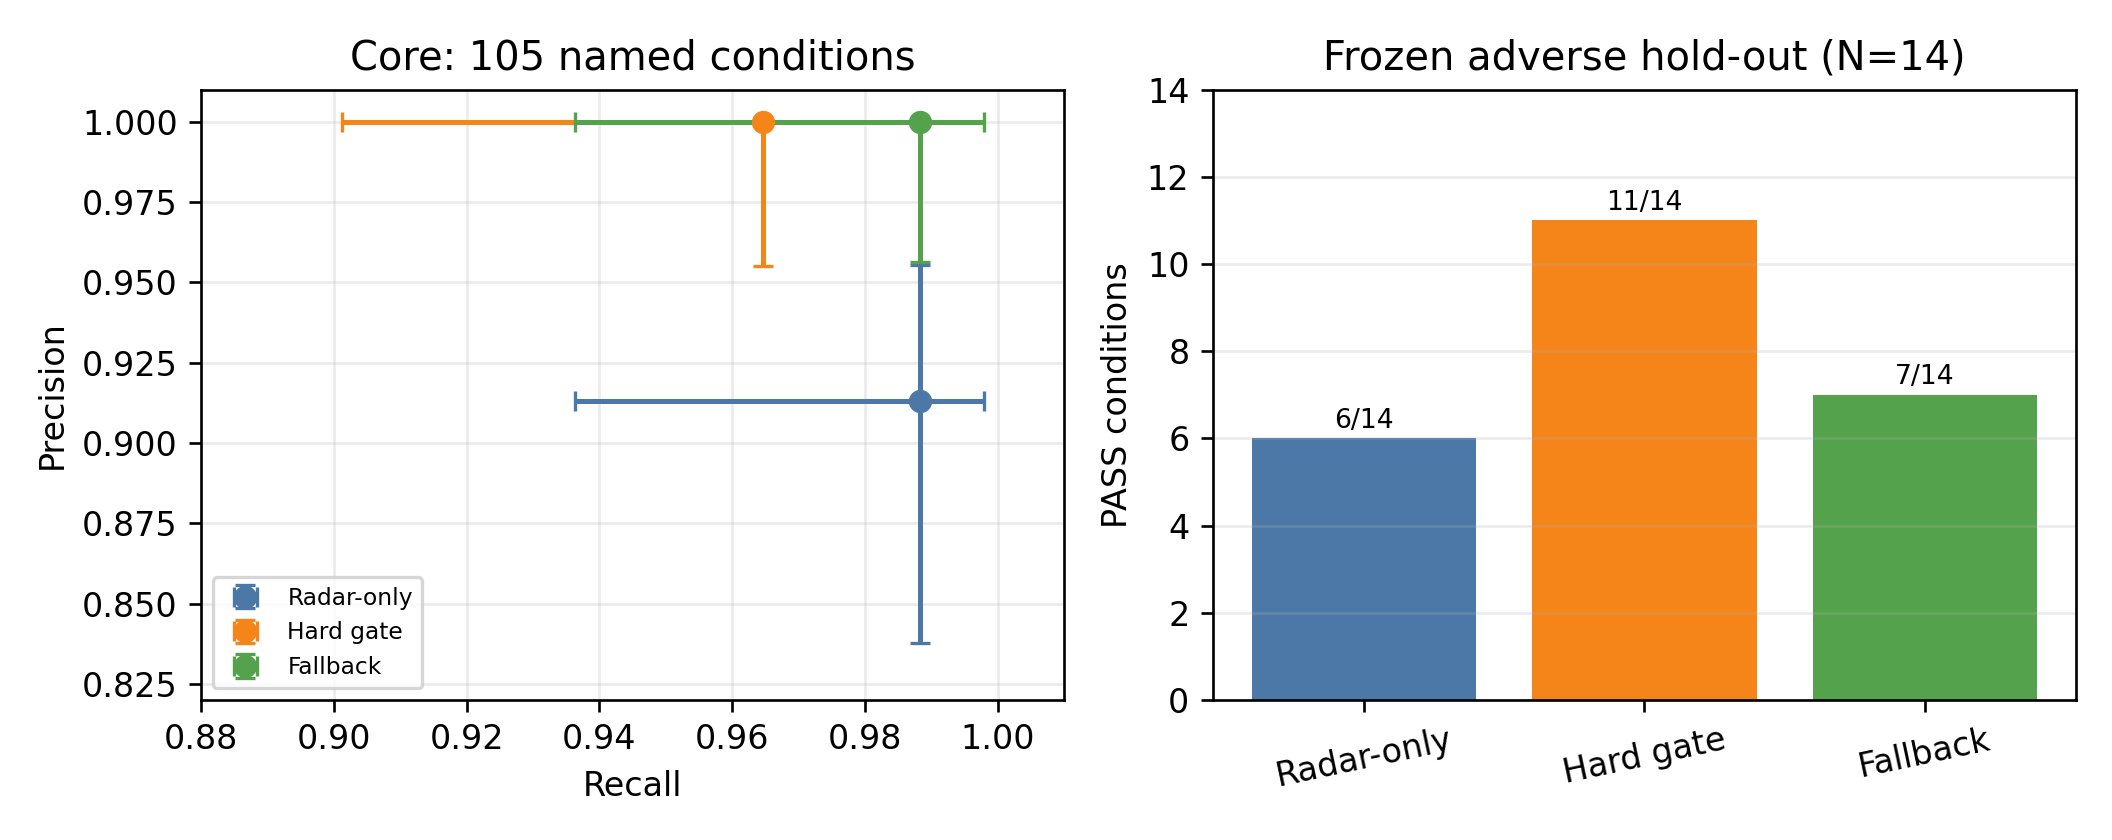
\includegraphics[width=0.92\textwidth]{scenario_level_tradeoff.png}
\caption{Bằng chứng named condition. Trái: core precision--recall với Wilson
interval mô tả. Phải: system PASS trên frozen adverse hold-out 14 điều kiện.
Không grid nào đại diện road prevalence.}
\label{fig:primary}
\end{figure*}

Hold-out đảo chiều apparent dominance. Nó gồm ba central props mới, bốn vehicle
appearances, hai edge props và năm persistent 6--10-point synthetic ghosts. Hard
gate một mình PASS bốn high-support ghost conditions; fallback một mình không
PASS điều kiện nào; cả hai PASS bảy và cùng FAIL ba. Fallback chỉ chặn ghost
offset 0,75~m. Ghost returns chủ ý tái tạo rule-level attributes của fallback,
nên đây là mechanism falsification test, không ước lượng real radar multipath
frequency. Label/injection geometry cố định trong YAML: closing virtual cluster
tồn tại gần predicted center path trong khi point count/offset vượt frozen
boundaries. Tên ``adverse mechanism hold-out'' tránh hàm ý independent deployment
distribution.

Vehicle appearances không phân tách hard gate/fallback vì camera label space vẫn
bao phủ. Physical props và ghosts mới tạo khác biệt. Decomposition theo mechanism
có ý nghĩa hơn aggregate F1: fallback thêm brake recall cho unlabelled track,
nhưng track-quality rule không có bằng chứng độc lập về physical existence.

\subsection{Phân rã mechanism}
Ba physical prop failures nằm ở các pipeline boundaries khác nhau. Shopping cart
cho tối đa hai path candidates nhưng không confirmed cluster; radar risk không
yêu cầu phanh và không late permission policy nào phục hồi được. Đây là radar
formation/representation failure, không phải chỉ camera veto. Bench tạo confirmed
track: radar-only phản ứng trước, fallback chờ point/path/TTC/margin đồng thời,
hard gate không có usable car confirmation. Traffic-warning lại khác: mọi policy
phanh cùng gap và camera-policy log cho confirmation thay vì fallback. Dù
permission sớm, configured vehicle/prop contact dynamics vẫn collision. Ba nhóm
là missing track, late emergency qualification và collision despite permission.

Ghost đi theo hướng ngược lại. Six-point center injection tạo một confirmed track
ở 0,15~s với confidence 1,0, TTC 0,89~s và margin $-15,21$~m; radar-only/fallback
lập tức emergency brake còn hard gate không có car confirmation. Ghost tám/mười
điểm center/offset 0,50~m tương tự. Dịch injection sang 0,75~m không đổi radar-only
nhưng vượt frozen path threshold 0,65~m của fallback. Adverse outcome vì vậy đi
trực tiếp từ rule, không phải YOLO timing chưa quan sát.

Regression FN cũng tách riêng. Trong năm repeats của late cut-out, radar target
rời/tái nhập predicted lateral corridor gần decision boundary và không policy
nào phanh. Gộp điều kiện này, high-speed stopping limits, unknown props và ghosts
thành một failure rate sẽ che mất stage có thể cải tiến.

\subsection{Ablation, sensitivity và controlled degradation}
Ablation development 12 điều kiện lặp hai lần cho full fallback 12/12. Hard gate
và no-latch cùng fail hai central box/barrel. Bỏ central-path tạo ba edge-prop
false-brake conditions; bỏ minimum point count tạo hai weak-ghost false brakes.
Bỏ stability/confidence hoặc đổi TTC-AND-margin thành OR không làm thay đổi focused
grid, nên không claim independent necessity. Trong sáu one-factor conditions,
giảm point count tạo một FP; tăng stability hoặc siết TTC mỗi loại bỏ một central
prop. Các local variants khác không đổi.

\begin{table}[t]
\caption{Kết quả extended theo named condition.}
\label{tab:extended}
\centering\scriptsize
\setlength{\tabcolsep}{3pt}
\begin{tabular}{llrrrrrrr}
\toprule Suite & Policy & Pass/N & TP & FP & TN & FN & Coll.\\ \midrule
Perturb. & Radar & 19/20 & 20 & 0 & 0 & 0 & 1\\
 & Hard & 15/20 & 15 & 0 & 0 & 5 & 5\\
 & Fallback & 18/20 & 20 & 0 & 0 & 0 & 1\\
\midrule
Camera off & Hard & 4/10 & 0 & 0 & 4 & 6 & 6\\
 & Fallback & 8/10 & 6 & 0 & 4 & 0 & 2\\
\bottomrule
\end{tabular}
\end{table}

Trong perturbation, box 19~m của fallback collision; box 21~m tránh collision
nhưng dừng ở 0,353~m, dưới criterion 0,5~m. Điều này sửa ambiguity khi coi mọi
system FAIL là collision. Khi camera off, fallback phanh cả sáu positives nhưng
collision hai; brake recall vẫn không đồng nghĩa safe stop. 4/10 PASS của hard
gate camera-off đều là TN, không phải hazard capability.

Các grid là one-factor local probes, không phải global threshold optimization.
Outcome không đổi với confidence, margin, path hoặc permissive TTC chỉ nghĩa sáu
conditions không qua boundaries đó, không chứng minh rule thừa. Ngược lại point,
path và latch ablations chủ ý chứa mechanism để phơi bày chúng; effect magnitude
vì vậy phụ thuộc suite.

\subsection{Failure severity và computation}
Bảng~\ref{tab:severity} tách ba physical mechanisms. Cart không có confirmed
radar cluster nên mọi policy impact không phanh ở 49,96~km/h. Bench có track:
radar-only phanh tại 12,62~m và last pre-impact tick 32,57~km/h; fallback đợi đến
4,29~m và đạt 54,93~km/h; hard gate không phanh và đạt 59,95~km/h. Với warning,
mọi policy phanh ở 21,87~m---gồm apparent camera confirmation---và đạt
7,82~km/h, cho thấy binary collision che mất mitigation lớn.

\begin{table}[t]
\caption{Failure severity trên hold-out (median của năm runs nhất quán).}
\label{tab:severity}
\centering\scriptsize
\setlength{\tabcolsep}{3pt}
\begin{tabular}{llrr}
\toprule Mechanism & Policy & Onset / gap & Severity outcome\\ \midrule
Cart & All & không phanh & pre-impact 49,96 km/h\\
Bench & Radar & 12,62 m & pre-impact 32,57 km/h\\
 & Hard & không phanh & pre-impact 59,95 km/h\\
 & Fallback & 4,29 m & pre-impact 54,93 km/h\\
Warning & All & 21,87 m & pre-impact 7,82 km/h\\
\midrule
Ghost FP & Radar (25 runs) & 78,4 km/h & 3,60 s / 9,02 m/s$^2$\\
 & Fallback (20) & 78,4 km/h & 3,60 s / 9,02 m/s$^2$\\
\bottomrule
\end{tabular}
\end{table}

Mọi ghost FP là full simulated stop dưới 1~km/h, không phải one-tick pulse; cột
cuối cho brake duration/peak deceleration ở hai dòng này. Điều đó làm binary
precision loss có ý nghĩa vận hành trong mô phỏng, dù không following-vehicle hay
occupant model nào chuyển thành crash risk. Ngược lại core system-limit collision
có pre-impact speed khoảng 20,43, 37,34 và 77,81~km/h dưới mọi policy, định vị
chúng downstream of gate. Bench còn cho nuance: radar-only vẫn binary FAIL nhưng
giảm 27,4~km/h so với hard gate; fallback phanh muộn chỉ giảm 5,0~km/h.

Trong 474 required-CUDA sessions, 74.928 inferences hoàn thành với 0 lỗi.
Session-median p50/p95 là 9,95/11,53~ms; weighted mean 11,56~ms. Mỗi process mới
có một cold start $>150$~ms; max 276,10~ms. Đây là ONNX host processing time
trong synchronous simulation, không end-to-end ECU deadline. Số này không gồm
radar preprocessing, callback transport, control application, display và vehicle
actuation. Cold event mỗi process được giữ vì process isolation là một phần
protocol.

\subsection{Traceability và audit}
Mỗi child summary ghi scenario/run ID, expected/actual brake, collision, minimum
gap, first brake time/speed/gap, target association, fallback reason và failure
text. Tick CSV thêm point, cluster, confidence, TTC, margin, command, provider và
collision state. Session manifest ghi commit, seed, CARLA client/server version,
model/config SHA-256, configured/active provider, inference count, errors và
latency quantiles. Checkpoint key là $(\mathrm{scenario\ id},\mathrm{run\ index})$,
nên technical retry thay run incomplete thay vì nhân đôi evidence. Derivation
script tái sinh named confusion, paired outcomes, collision severity và false-
brake severity từ frozen archive mà không đổi run.

\section{Thảo luận và biên hiệu lực}
\subsection{Hàm ý thiết kế}
Các policy mã hóa error cost khác nhau. Hard gating bảo thủ khi car-only detector
bao phủ hazard nhưng có cấu trúc từ chối unlabelled object. Fallback phục hồi một
phần radar recall đồng thời nhận stable/central/high-support ghosts. Track age,
point count, confidence, path offset, TTC và margin đều là thuộc tính của một
radar estimate; không thuộc tính nào độc lập chứng minh physical existence.
Threshold tuning chỉ dịch operating point và có thể làm genuine brake muộn như
bench, sensitivity và camera-off cho thấy. Cần bằng chứng mới---free space,
semantics rộng hơn, occupancy, calibrated existence probability hay radar cue
phong phú---để phá symmetry.

Policy choice cần theo error cost rõ. Khi unnecessary high-deceleration braking
là cost chính, hard gate được ưu tiên trên grid này; khi camera availability hay
non-vehicle recall quan trọng, fallback phục hồi một phần nhưng cần existence
model mạnh hơn. Radar-only là upper envelope hữu ích cho request của shared radar
risk stage, không phải road-ready policy. Failure severity phải đi cùng confusion:
warning cho collision mitigation dù system FAIL, trong khi ghost cho thấy một FP
có thể là complete emergency stop.

\subsection{Biên hiệu lực}
Điểm mạnh là controlled substitution và adverse evidence, không phải algorithmic
novelty rộng. Bài báo chưa so sánh learned/probabilistic fusion, confidence-matched
soft gate hay multi-class/free-space perception. External validity giới hạn bởi
một map/ego, một fixed seed, favorable imaging, dataset in-domain tách session,
point-level CARLA radar và deterministic repeats. Synthetic ghost được xây dựng
chủ ý, không phải measured multipath distribution. Adverse hold-out chỉ có 14
conditions; interval rộng thể hiện giới hạn. Không có weather/friction sweep,
HIL, actuator/communication delay, real radar/camera data hay vehicle test.
False-brake duration/deceleration và last-tick pre-impact speed cải thiện binary
report nhưng không phải occupant-risk hoặc jerk-cost model. Scenario không chứng
nhận ISO hay Euro NCAP compliance.

Mọi child run lưu commit, seed, model/config SHA-256, CARLA version, active
provider và tick-level gate reason. Raw CSV/JSON, snapshot, manifest, derivation
script và archive SHA-256 tái tạo run/scenario-level result. Đây là auditability,
không road-population inference.

Protocol tiếp theo nên pre-register stochastic fault surface thay vì một ghost
hướng threshold: point support 4--12, offset 0--1~m, persistence, range-rate
noise, intermittent returns qua nhiều seeds. Cần thêm map, weather/illumination,
friction và ego platform thứ hai. Policy cạnh tranh nên có confidence-matched
soft gate, multi-class/free-space evidence và probabilistic existence tracker.
Evaluation giữ named-condition pairing nhưng thêm impact speed, brake duration,
jerk-aware false-brake cost và time-to-last-safe-brake. Recorded/HIL radar sau đó
mới kiểm tra mechanism map có chuyển ra ngoài CARLA abstraction hay không.

\section{Kết luận}
Trên core grid đã xây dựng, emergency fallback kết hợp hard-gate precision và
radar-only recall. Trên frozen adverse hold-out, hard gate PASS nhiều hơn vì
fallback nhận synthetic ghosts thuyết phục, trong khi mọi policy còn failure do
missing/late physical track. Scenario-level statistics và severity làm lộ thông
tin bị run total lặp và binary collision che mất. Camera gating vì vậy là cơ chế
false-positive suppression và radar emergency fallback là conditional
trade-off---không policy nào là general safety solution.

\balance
\bibliographystyle{IEEEtran}
\bibliography{references}
\end{document}
